\section {Применение имитационного моделирования в теории массового обслуживания}
Имитационное моделирование является мощным инструментом для изучения сложных систем массового обслуживания. Его актуальность обусловлена следующими факторами:
\begin{enumerate}
	\item Принцип, лежащий в основе моделирования, довольно прост для понимания, что делает этот инструмент доступным для широкого круга исследователей, в том числе для тех, кто не имеет глубоких познаний в теории случайных процессов;
	\item При использовании имитационного моделирования в связке со сложными средствами визуализации можно детально наблюдать процесс работы системы в различных ее аспектах, что дает данные, которые невозможно получить при помощи исключительно численного подхода к анализу, более сфокусированного на различных показателях функционирования системы; 
	\item Численные методы в большинстве случаев опираются на решение специально составленных систем уравнений (система уравнений Колмогорова). В свою очередь, имитационное моделирование предлагает методологию, которая помогает рассчитать те же показатели без изменения основного подхода \cite{glynn1988simulation};
\end{enumerate}

Как упомянуто выше, ключевое преимущество имитационного моделирования --- прямолинейная реализация алгоритма, что экономит время и снижает трудоемкость исследования.

При моделировании систем массового обслуживания используется дискретно-событийный подход. Он заключается в генерации случайных величин, имеющих требуемое распределение, которые являются моментами наступления событий в системе. События могут быть различного рода: окончание обслуживания заявки, перемещение заявки на прибор, поломка прибора и т. д. В момент наступления события состояние системы меняется, что и отслеживается в процессе моделирования.

Рассмотрим подход подробнее на примере следующей системы:

на вход системы поступает пуассоновский поток заявок. Заявка занимает прибор в случае, если он свободен, тот, в свою очередь, начинает ее обслуживание в течение экспоненциально распределенного времени с параметром $\mu$. В ситуации, когда прибор уже занят обслуживанием, входящая заявка, после неудавшейся попытки захватить прибор, мгновенно уходит на орбиту и осуществляет там случайную задержу в течение экспоненциально распределенного времени с параметром $\sigma$.

\begin{figure}[H]
	\centering
	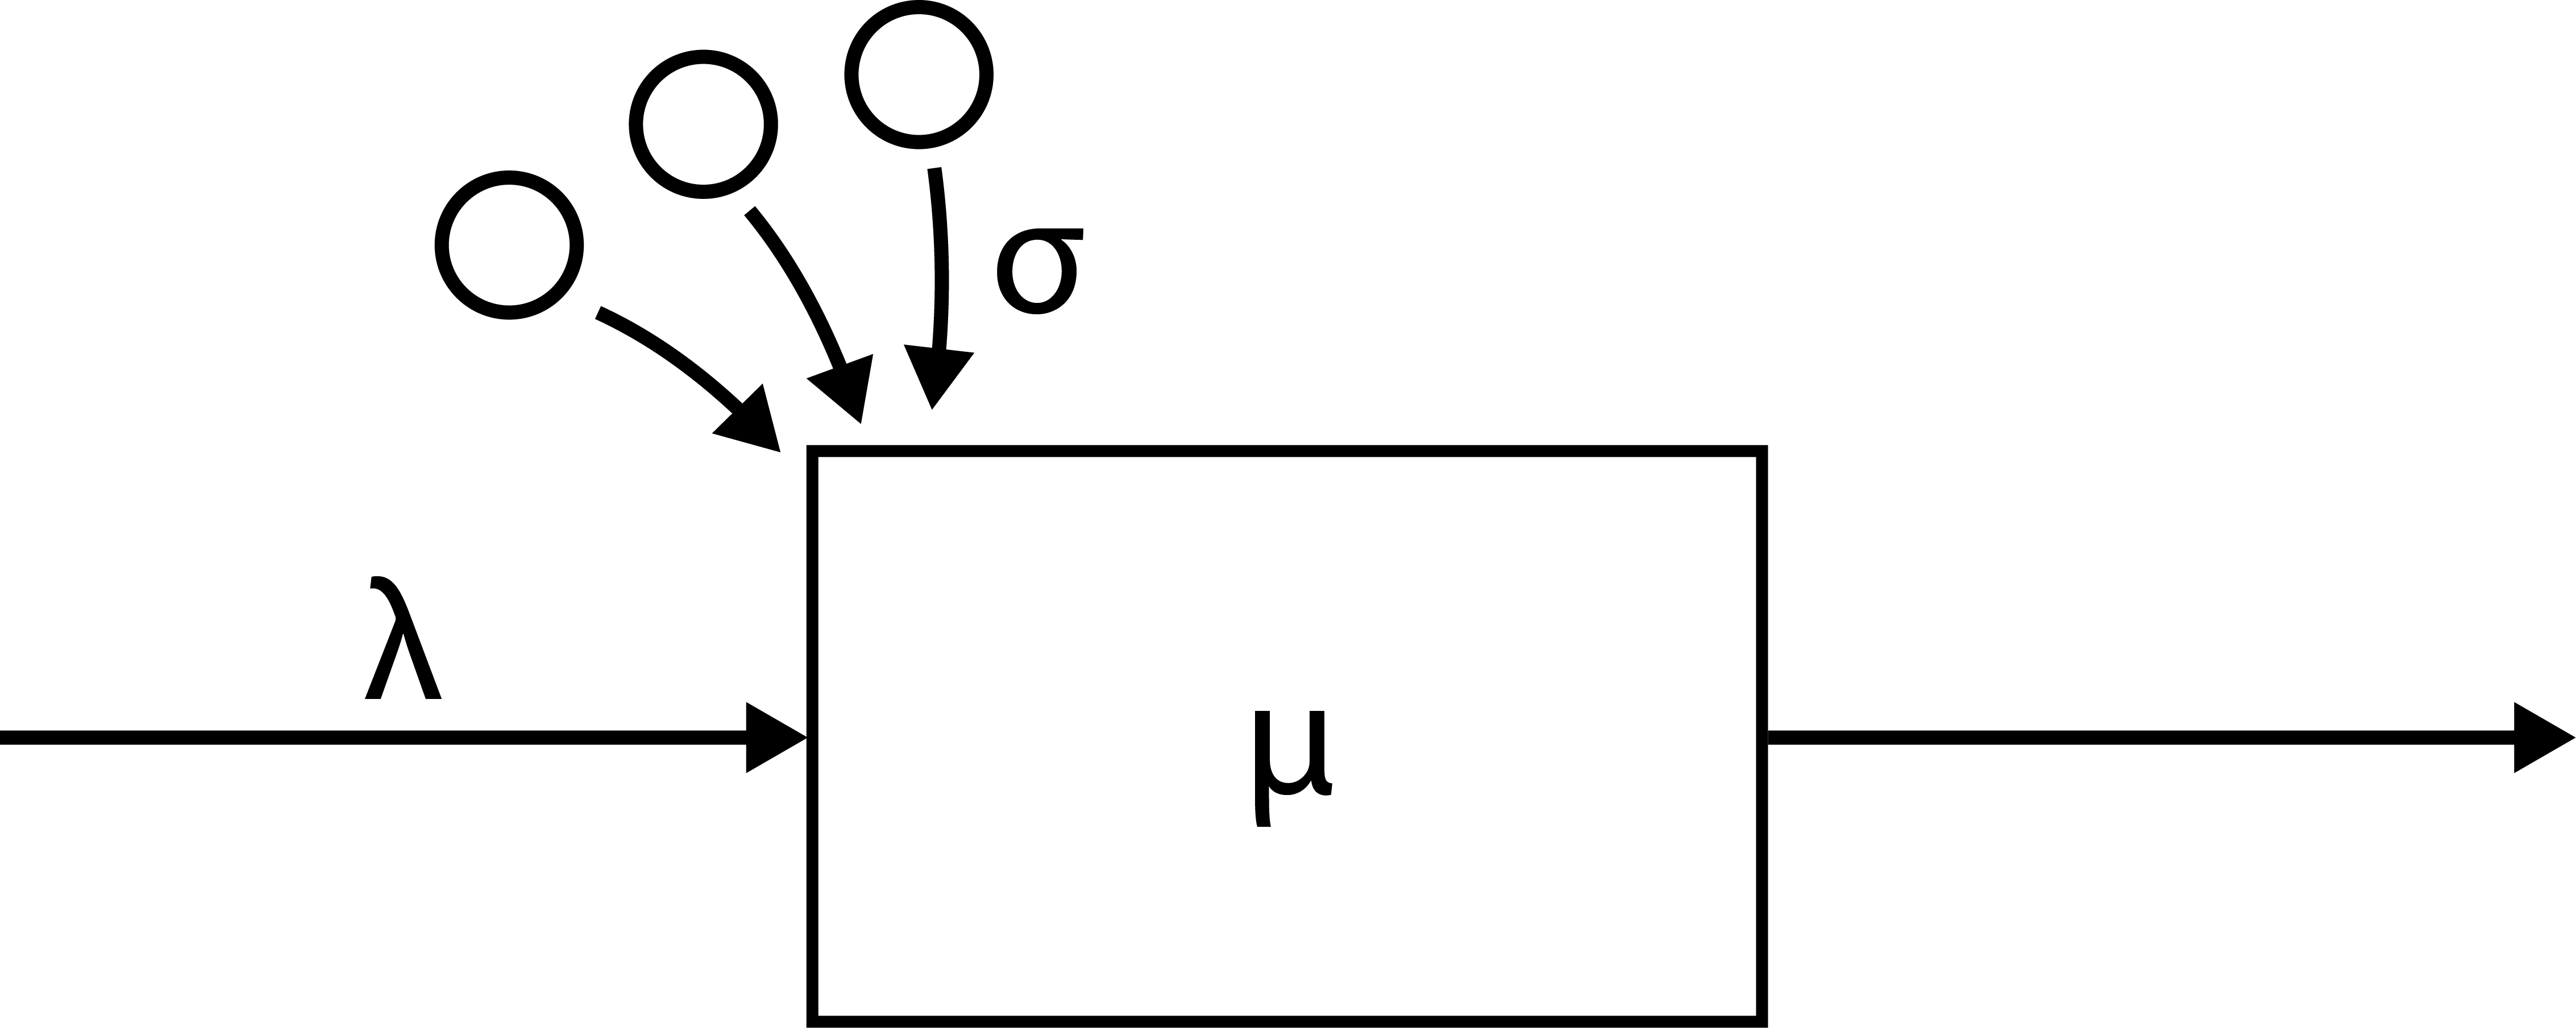
\includegraphics[scale=1,width=\textwidth]{1_sim_example.png}
	\caption{Пример системы ТМО}
	\label{sys_tmo_example}
\end{figure}

Введем следующие обозначения: $i(t)$ --- число заявок на орбите в момент времени $t$, $k(t)$ --- состояние прибора: $0$ --- прибор свободен, $1$ --- прибор занят обслуживанием заявки входящего потока, $m_1(t)$ --- количество обслуженных заявок входящего потока в момент времени $t$.

Помимо этого введем следующие обозначения:
%\begin{enumerate}
	
%\end{enumerate}